\subsection{Universal Asynchronous Receiver Transmitter}
En UART er en enhed, der implementerer seriel data og er dermed et led mellem et parallelt og et serielt interface, der både modtager og sender data. Data sendes som bits og kan både sendes serielt eller parallelt. \citep{Jimb02016a,Chun-zhiYin-shuiLun-yao2011} Parallelt bliver flere bits overført på samme tid, hvormed et 8-bit system er nødsaget til at have otte ledninger, hvor der i den ene ende er en RX kobling og i den anden er en TX kobling. \citep{Jimb02016a} Den serielle kommunikation foregår asynkront og kan foregå med én ledning, da kun en bit overføres af gangen. Den serielle kommunikation benyttes oftest, da der ikke kræves så mange ledninger. Det er i den serielle kommunikation nødvendigt at bestemme en baudrate\fxnote{baudrate = Hvor hurtigt der sendes data (bits per sekund[bps])}, som TX og RX synkroniseres efter. Det modtagne data gemmes ofte i en buffer, som efterfølgende videregives i form af first-in-first-out (FIFO). \citep{Jimb02016a}\newline 
Overførsel af data sker asynkront, som det ses på \figref{fig:asynkron}.
\begin{figure}[H]
	\centering
	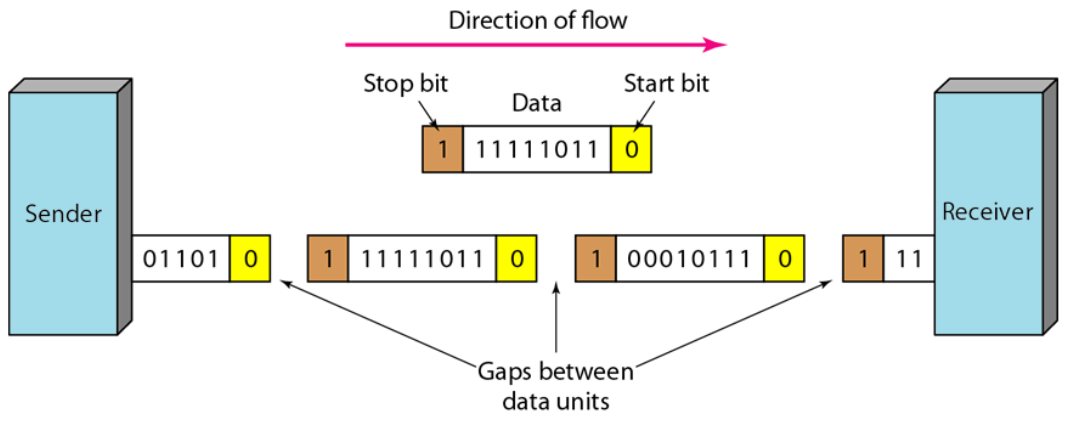
\includegraphics[scale=0.5]{figures/bProblemloesning/asynkron.png}
	\caption{På figuren ses en asynkron dataoverførsel mellem en afsender TX og en modtager RX. Dataenhederne sendes ved brug af et start- og stopbit for alle afsendte enheder. \citep{Jimb02016} (Modificeret)}
	\label{fig:asynkron}
\end{figure}\vspace{-0.25cm}
Ved denne kommunikationsform opererer RX og TX ved to forskellige clocks. For at opnå synkront data sættes et startbit og stopbit\fxnote{alt udenfor disse overføres ikke}, hvilket illustreres på \figref{fig:asynkron}. Data i gaps mellem stop- og startbit kasseres. UARTens opgave er at læse parallel data fra FIFO, som laves om til seriel data. Dette data kan efterfølgende sendes til andre enheder. Når RX i en anden enhed modtager et startbit, laves data om fra seriel til parallel data, hvorefter data kan skrives til modtager-FIFO. \citep{Jimb02016a,Chun-zhiYin-shuiLun-yao2011}

Nogle enheder indeholder mere end én seriel-linje, og disse enheder fungerer enten som fuld-duplex eller halv-duplex. Fuld-duplex enheder kan både sende og modtage data på samme tid. Halv-duplex enheder sender og modtager data på skift. \citep{Jimb02016a,Chun-zhiYin-shuiLun-yao2011}